\chapter{\ifproject%
\ifenglish Project Structure and Methodology\else โครงสร้างและขั้นตอนการทำงาน\fi
\else%
\ifenglish Project Structure\else โครงสร้างของโครงงาน\fi
\fi
}

ในบทนี้จะกล่าวถึงหลักการ และการออกแบบระบบ

\makeatletter

% \renewcommand\section{\@startsection {section}{1}{\z@}%
%                                    {13.5ex \@plus -1ex \@minus -.2ex}%
%                                    {2.3ex \@plus.2ex}%
%                                    {\normalfont\large\bfseries}}

\makeatother
%\vspace{2ex}
% \titleformat{\section}{\normalfont\bfseries}{\thesection}{1em}{}
% \titlespacing*{\section}{0pt}{10ex}{0pt}
% \begin{figure}
% \begin{center}
% 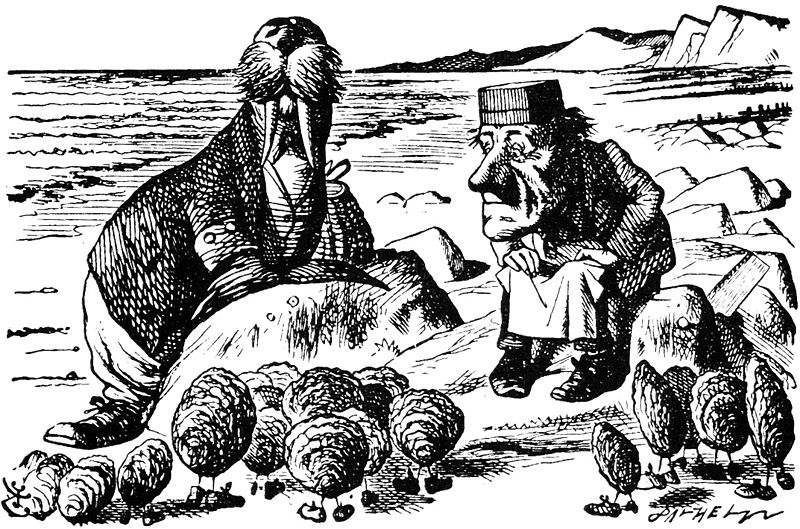
\includegraphics{photo/800px-Briny_Beach.jpg}
% \end{center}
% \caption[Poem]{The Walrus and the Carpenter}
% \label{fig:walrus}
% \end{figure}

\section{ภาพรวมของแอพพลิเคชัน}

เว็บแอพพลิเคชันจะเป็นแบบ three-tier architecture แต่ว่าจะทำการออกแบบ และพัฒนาให้สามารถรองรับการเปลี่ยนแปลงเป็น 
microservice ได้ โดย Front-end และ Back-end ส่วนมากจะพัฒนาด้วย Next.js และ tRPC เพื่อความสะดวกสบายในการเรียกใช้งาน API
และใช้ typescript ให้มีประสิทธิภาพ แต่ Back-end ในส่วนของระบบจับคู่นั้นจะพัฒนาด้วย Go เพราะสามารถเขียน concurrency ได้ง่ายแต่ยังคงไว้ซึ่งประสิทธิภาพ
ส่วนสุดท้ายคือฐานข้อมูลจะใช้ postgresql ในการจัดเก็บและติดต่อกับ Back-end ทั้ง Next.js และ Go

% เว็บแอพพลิเคชันใช้ three-tier architecture~\cite{ttarch} ในการออกแบบระบบ โดย front-end ใช้ Next.js\cite{nextjs} 
% ที่เป็น React~\cite{react} framework ส่วน back-end ใช้ Gin Gonic~\cite{gingonic} ซึ่งเป็น Go~\cite{golang} framework ติดต่อกับ Front-end 
% ด้วย GraphQL~\cite{graphql} API และฐานข้อมูลใช้ MySQL~\cite{mysql} เป็น relational database management system (RDBMS)

\begin{figure}[h]
\begin{center}
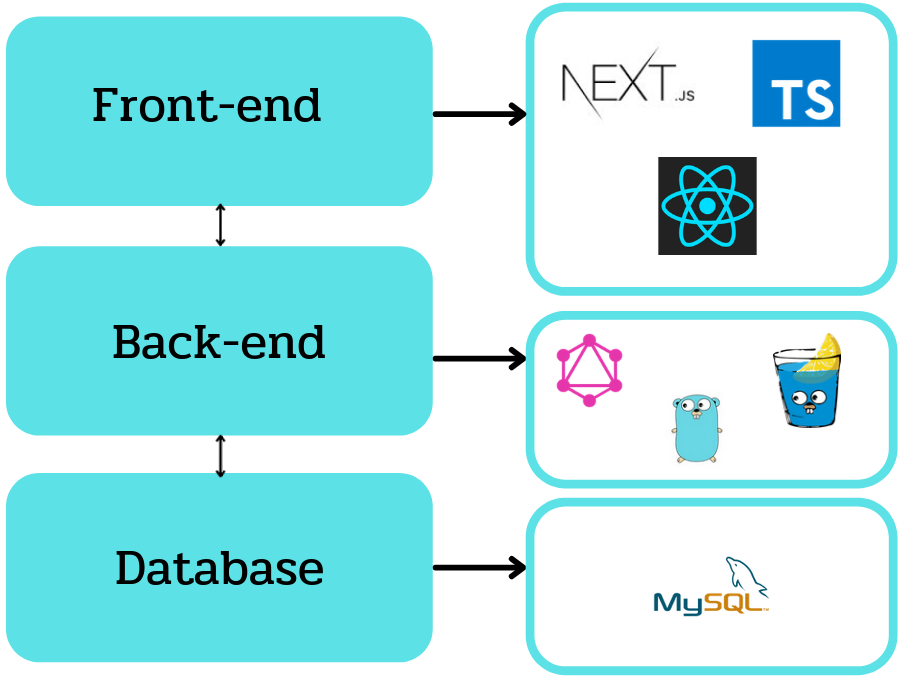
\includegraphics[width=2.5in]{photo/threetierarch.png}
\end{center}
\caption{three-tier architecture}
\label{fig:three-tier}
\end{figure}

\section{วิธีการจับคู่}
\begin{enumerate}
  \item นำลำดับคุณลักษณะที่ผู้ใช้ $u$ จัดอันดับไปแปลงเป็นตัวเลขเพื่อใช้เป็นตัวคูณในขั้นตอนต่อๆไป โดยเรียกตัวคูณนั้นว่า $\mathit{mult}$
  \item เก็บรายการคุณลักษณะที่ผู้ใช้พิจารณาเพื่อนร่วมห้องจากการจัดลำดับในขั้นตอนก่อนหน้าแล้วเรียกว่า $\mathit{attr}$
  \item ปรับปรุง $\mathit{mult}$ เพิ่มเติมในขั้นตอนการปรับจูน หากคุณลักษณะใดที่ผู้ใช้ให้ความสนใจบ่อยๆ จะถูกเพิ่มค่าให้มากขึ้น และคุณลักษณะใดที่ผู้ใช้ไม่ให้ความสนใจก็จะถูกลดค่าให้น้อยลง 
        เช่น หากมีโปรไฟล์ที่มีคุณลักษณะดังนี้
        \begin{enumerate}
          \item เวลานอนช่วง 4 ทุ่ม -- 5 ทุ่ม และ เป็นคนช่างพูด  
          \item เวลานอนช่วง 4 ทุ่ม -- 5 ทุ่ม และ เป็นคนพูดน้อย  
        \end{enumerate} 
        แล้วผู้ใช้เลือกทั้งสองโปรไฟล์นั้น ดังนั้นระบบจะทำการปรับเพิ่มค่าในตัวคูณของคุณลักษณะเวลานอนใน $\mathit{mult}$
  \item นำ $\mathit{mult}$ ไปคูณกับค่าของคุณลักษณะของผู้ใช้ $v$ คนอื่นๆที่ไม่ใช่ $u$ แล้วบวกผลคูณทั้งหมดเข้าด้วยกัน เรียกว่า $\mathit{RoommatePref}$
  \item ทำแบบข้อก่อนหน้ากับคุณลักษณะของห้องพักที่ต้องการ และ คุณลักษณะตามโปรไฟล์ของผู้ใช้ $u$ เรียกว่า $\mathit{RoomPref}$ และ $\mathit{PersonalPref}$ ตามลำดับ
  \item สร้างคู่อันดับ $(\mathit{RoomPref}, \mathit{RoommatePref})$ จากค่าของผู้ใช้ เรียกว่า $(x,y)$ 
  \item สร้างคู่อันดับ $(\mathit{RoomPref}, \mathit{PersonalPref})$ ของผู้ใช้คนอื่น เรียกว่า $(x',y')$
  \item หาคู่อันดับ $(x',y')$ ที่มีระยะทางแบบยูคลิด~\cite{euclid-dist} จาก $(x,y)$
  \[\sqrt{(x-x')^2 + (y-y')^2}\] มีค่าน้อยที่สุด 
  แล้วให้ $(x',y')$ ของผู้ใช้คนนั้นคู่เป็นเพื่อนร่วมห้อง
\end{enumerate}

\section{Features}
ต่อไปจะเป็นการอธิบายการทำงานของระบบในส่วนต่างๆ ทั้งฝั่งผู้ใช้งานทั่วไปและผู้ดูแลระบบ โดยรูปภาพตัวอย่างต่อไปนี้เป็นเพียง wireframes เท่านั้น ไม่ใช่ user interface ของระบบจริง
\subsection{End-user}
\begin{enumerate}
\item ระบบยืนยันตัวตน: ให้ผูู้ใช้ลงทะเบียนสมัครสมาชิกและเข้าสู่ระบบเพื่อที่จะสามารถใช้งานระบบต่างๆของระบบได้ต่อไป
\begin{figure}[h]
\begin{center}
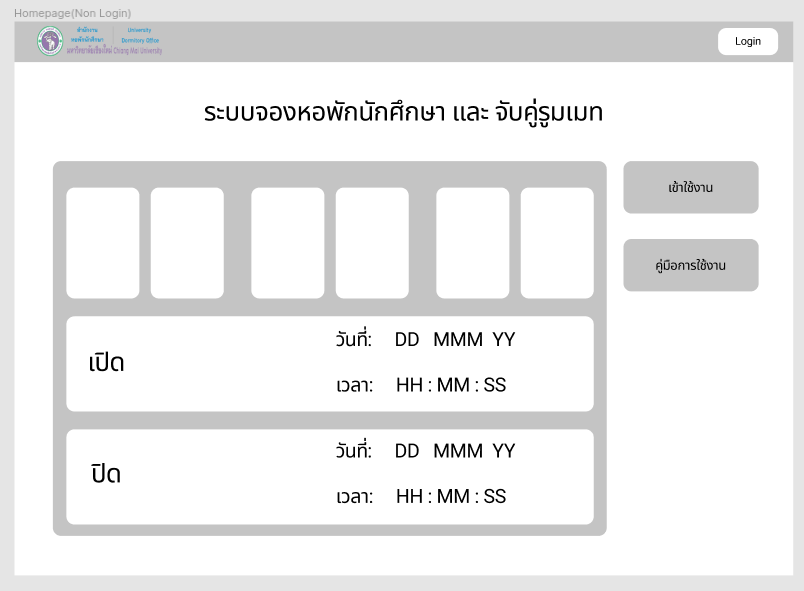
\includegraphics[width=\linewidth]{photo/homepageNoAuth.png}
\end{center}
\caption{homepage ที่ผู้ใช้ยังไม่ได้เข้าสู่ระบบ}
\label{fig:hp-no-auth}
\end{figure}

  \begin{figure}[h]
  \begin{center}
  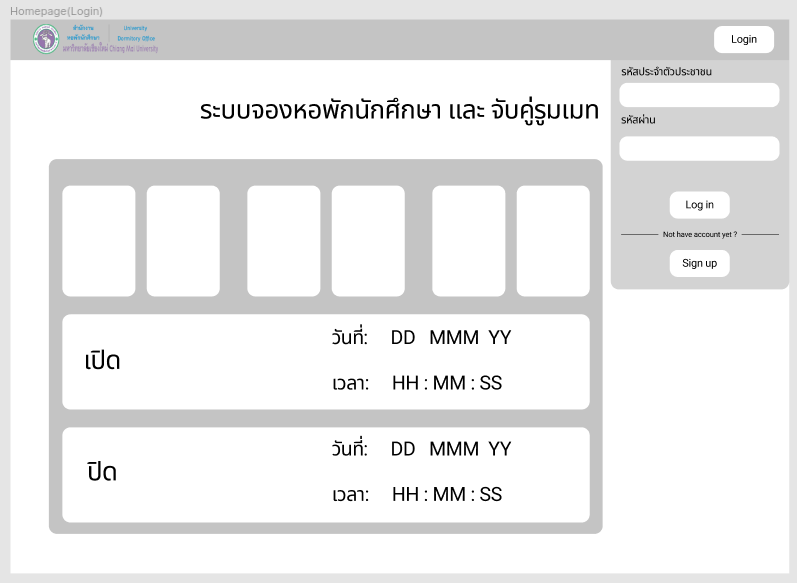
\includegraphics[width=\linewidth]{photo/homepageLogin.png}
  \end{center}
  \caption{homepage ขณะกำลังจะเข้าสู่ระบบ}
  \label{fig:hp-login}
  \end{figure}

  \begin{figure}[h]
  \begin{center}
  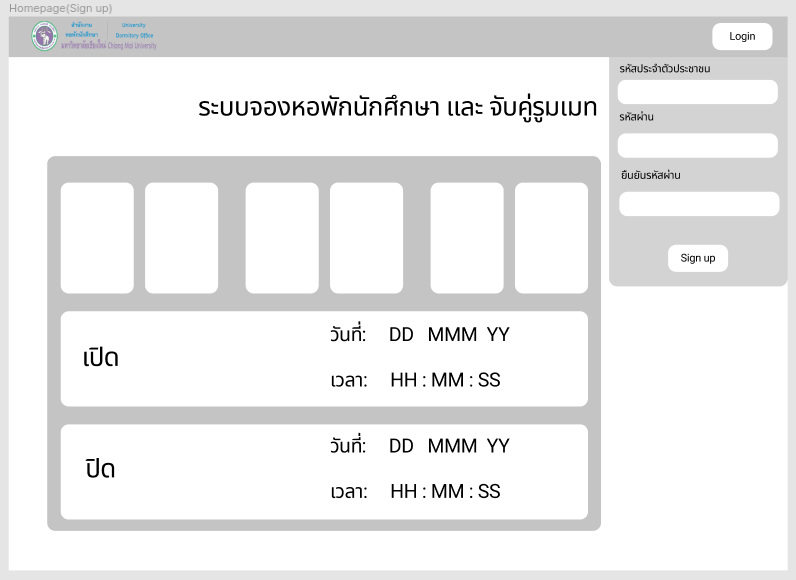
\includegraphics[width=\linewidth]{photo/homepageReg.png}
  \end{center}
  \caption{homepage ที่ผู้ใช้กำลังสมัครสมาชิก}
  \label{fig:hp-reg}
  \end{figure}

  \begin{figure}[h]
  \begin{center}
  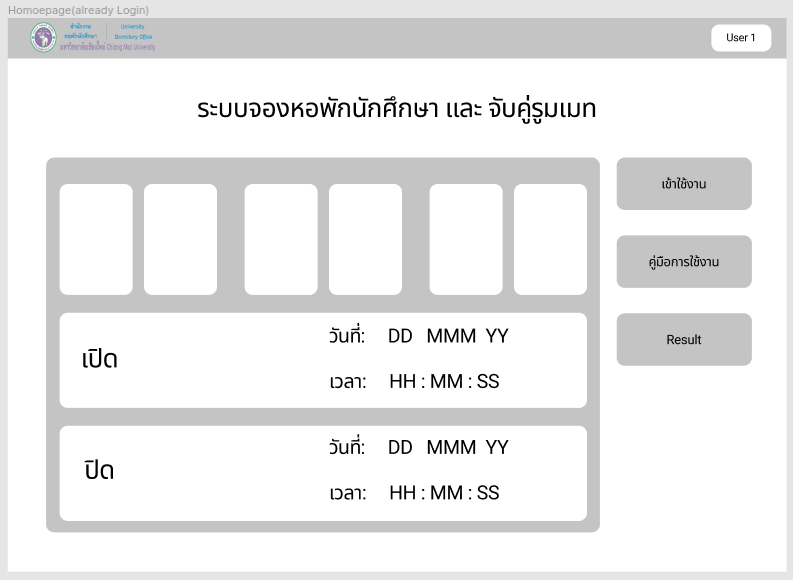
\includegraphics[width=\linewidth]{photo/homepageAuth.png}
  \end{center}
  \caption{homepage ที่ผู้ใช้เข้าสู่ระบบแล้ว}
  \label{fig:hp-auth}
  \end{figure}

  \clearpage
  \item ระบบการจัดอันดับคุณลักษณะ: ให้ผู้ใช้ที่ลงชื่อเข้าใช้แล้วเลือกคุณสมบัติของห้องและเพื่อนร่วมห้องที่ต้องการ
  \begin{figure}[h]
  \begin{center}
  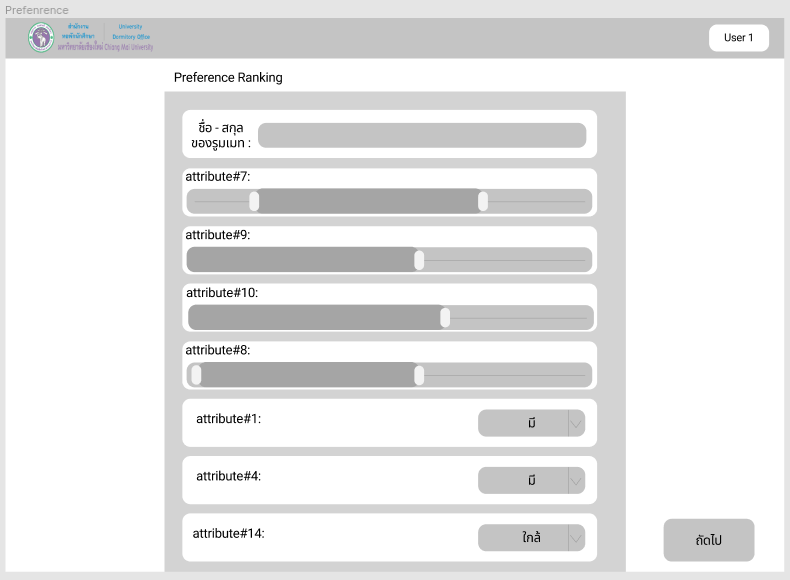
\includegraphics[width=\linewidth]{photo/Preference.png}
  \end{center}
  \caption{หน้า preference ให้ผู้ใช้เลือกคุณลักษณะที่ต้องการ}
  \label{fig:preference}
  \end{figure}
  
  \clearpage
  \item ระบบปรับจูนคุณลักษณะ: ระบบจะทำการนำโปรไฟล์ของบุคคลอื่นๆ มาแสดงให้ผู้ใช้เลือกว่า หากเป็นบุคคลที่มี
  คุณลักษณะตามโปรไฟล์ ผู้ใช้จะเลือกบุคคลดังกล่าวเป็นเพื่อนร่วมห้องหรือไม่ เพื่อคำนวณหาระดับความใส่ใจในคุณลักษณะต่างๆของผู้ใช้ 
  ตัวอย่างดังรูปที่~\ref{fig:finetune}
  \begin{figure}[h]
  \begin{center}
  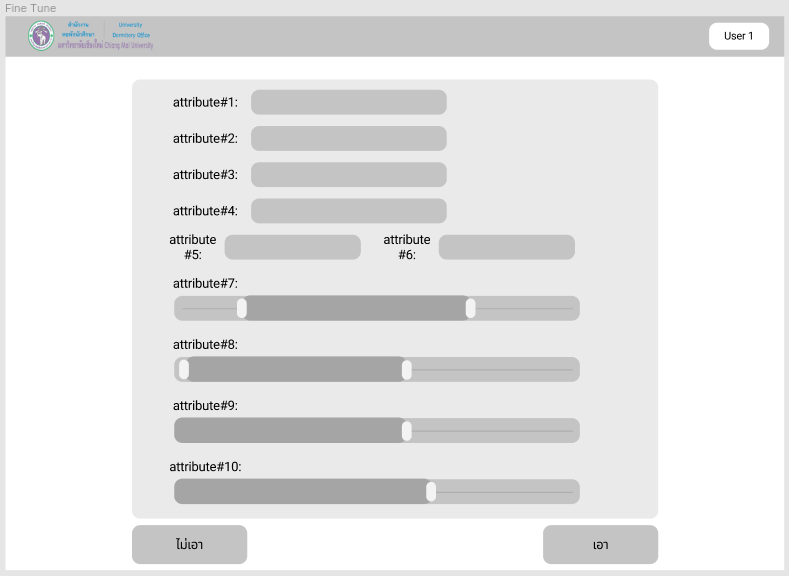
\includegraphics[width=\linewidth]{photo/finetune.png}
  \end{center}
  \caption{หน้า fine tune}
  \label{fig:finetune}
  \end{figure}

  \clearpage
  \item ระบบรายงานสรุปผล: แสดงความคืบหน้าว่า ณ ปัจจุบันผู้ใช้มีโอกาสจะได้จับคู่กับเพื่อนร่วมห้องที่มีคุณลักษณะอย่างไร 
        และจะได้ห้องแบบใด 
  \begin{figure}[h]
  \begin{center}
  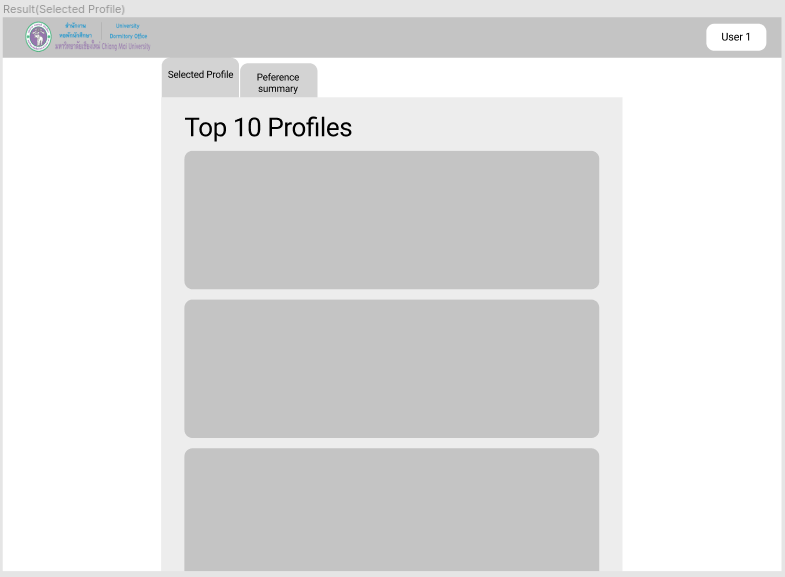
\includegraphics[width=\linewidth]{photo/resultSelectedProfile.png}
  \end{center}
  \caption{หน้าสรุปผล 10 อันดับสูงสุดที่มีโอกาสได้จับคู่กับผู้ใช้}
  \label{fig:select-profile}
  \end{figure}
  \begin{figure}[h]
  \begin{center}
  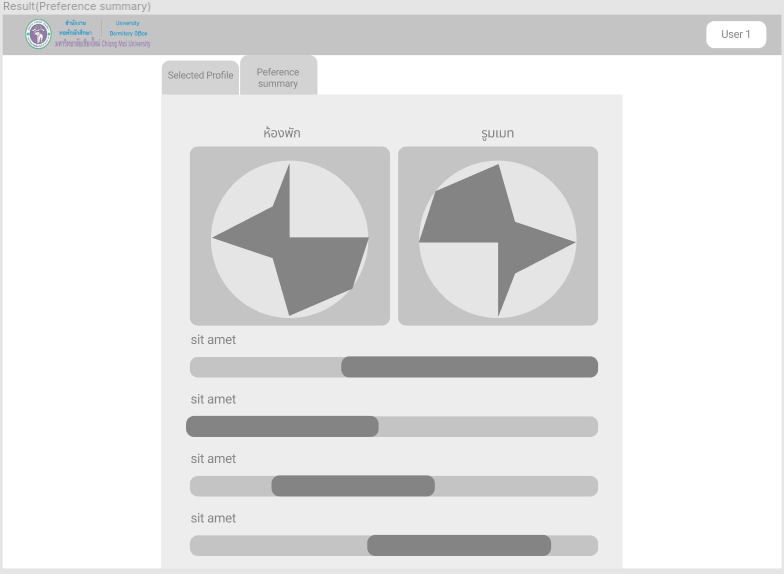
\includegraphics[width=\linewidth]{photo/resultPreferenceSummary.png}
  \end{center}
  \caption{หน้าสรุปผลคุณลักษณะที่ผู้ใช้ให้ความสนใจ}
  \label{fig:summary}
  \end{figure}

  \clearpage
  \item ระบบคู่มือการใช้งาน: แสดงคู่มือการใช้งานของระบบสำหรับผู้ใช้ทั่วไป ไม่รวมผู้ใช้ที่เป็นผู้ดูแลระบบ
  \begin{figure}[h]
  \begin{center}
  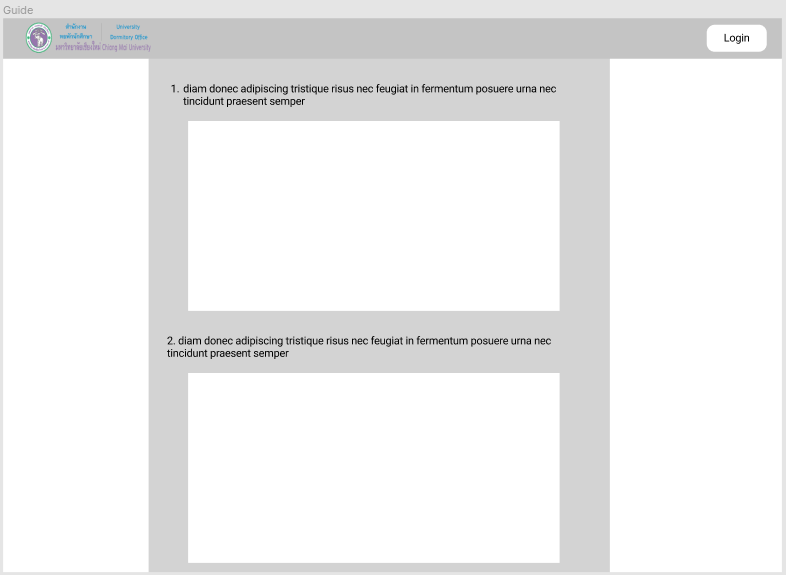
\includegraphics[width=\linewidth]{photo/Guideline.png}
  \end{center}
  \caption{หน้าคู่มือการใช้งาน}
  \label{fig:guideline}
  \end{figure}

  \clearpage
  \item ระบบโปรไฟล์ผู้ใช้: ให้ผู้ใช้เข้าไปปรับแต่งคุณลักษณะของตนเองเพื่อนำไปใช้ในการจับคู่กับผู้อื่น
  \begin{figure}[h]
  \begin{center}
  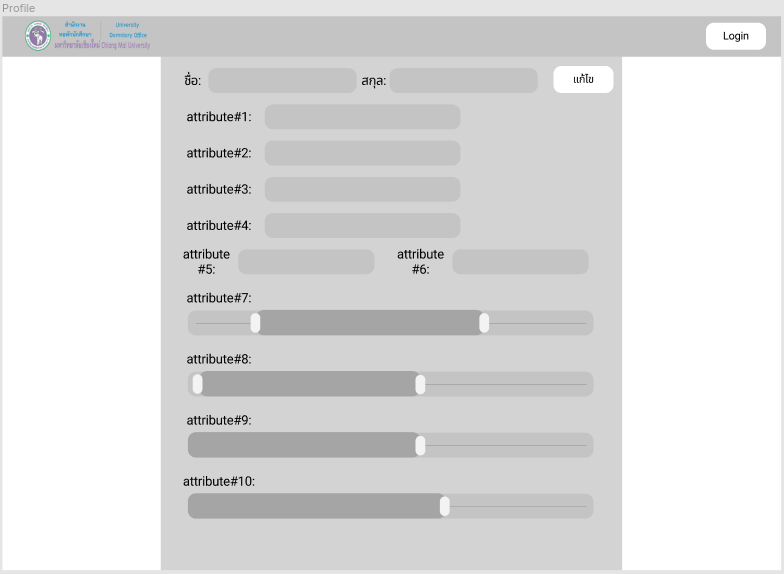
\includegraphics[width=\linewidth]{photo/profile.png}
  \end{center}
  \caption{หน้าโปรไฟล์}
  \label{fig:profile}
  \end{figure}
  
\end{enumerate}

\subsection{Administrator}
\begin{enumerate}
  \item ระบบจัดการเวลาเปิด--ปิดวันลงทะเบียน: ให้ผู้ดูแลระบบสามารถตั้งค่าเวลาเปิด--ปิด
  วันลงทะเบียนของผู้ใช้ทั่วไป
  \begin{figure}[h]
  \begin{center}
  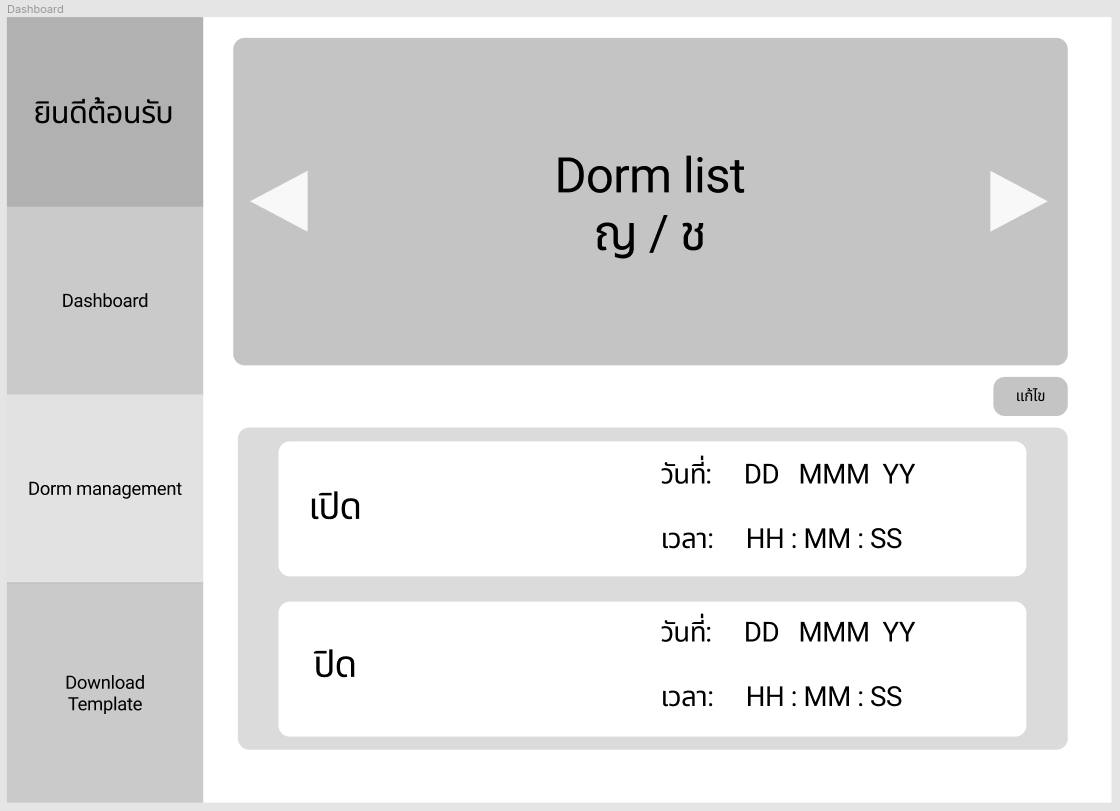
\includegraphics[width=\linewidth]{photo/adminDashboard.png}
  \end{center}
  \caption{หน้า homepage ของผู้ดูแลระบบ}
  \label{fig:dashboard}
  \end{figure}
  \begin{figure}[h]
  \begin{center}
  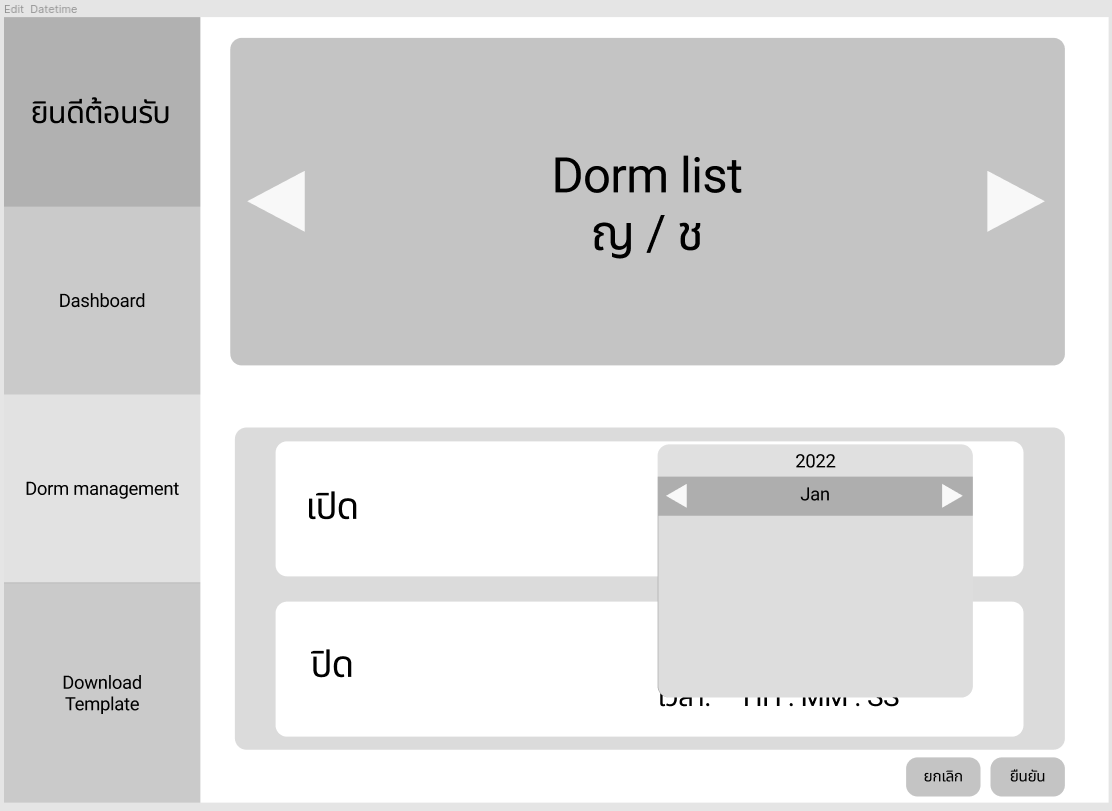
\includegraphics[width=\linewidth]{photo/datepicker.png}
  \end{center}
  \caption{ตัวอย่างการเปลี่ยนวันที่เปิด--ปิดระบบ}
  \label{fig:datepicker}
  \end{figure}
  \begin{figure}[h]
  \begin{center}
  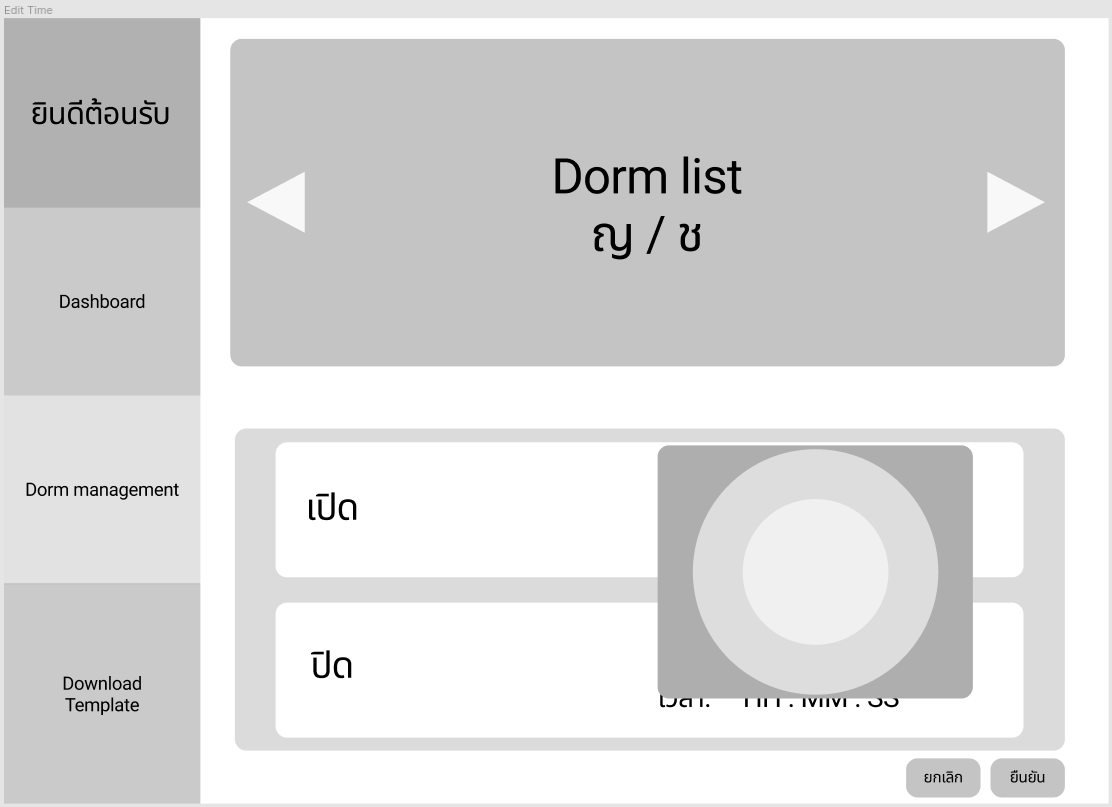
\includegraphics[width=\linewidth]{photo/timepicker.png}
  \end{center}
  \caption{ตัวอย่างการเปลี่ยนเวลาที่เปิด--ปิดระบบ}
  \label{fig:timepicker}
  \end{figure}
  \begin{figure}[h]
  \begin{center}
  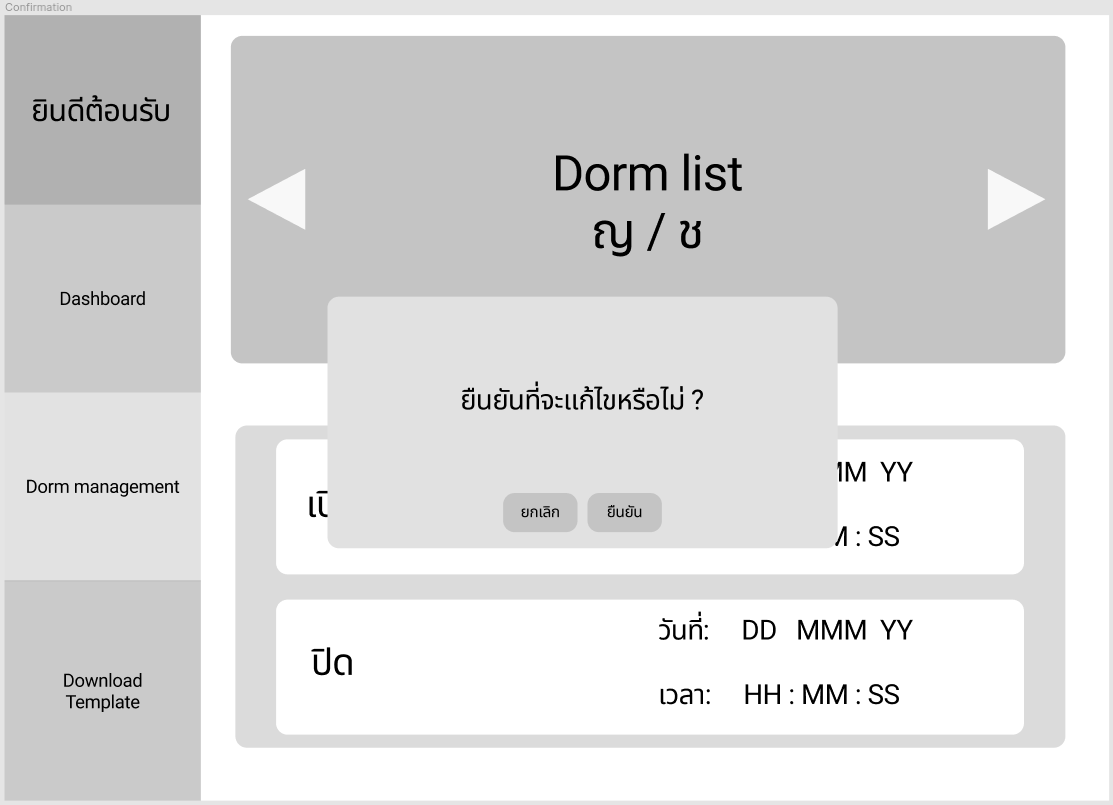
\includegraphics[width=\linewidth]{photo/confirmation.png}
  \end{center}
  \caption{ตัวอย่างแจ้งเตือนเพื่อยืนยันการตั้งค่า}
  \label{fig:confirm-date-time}
  \end{figure}

  \clearpage
  \item ระบบจัดการฐานข้อมูลและการตั้งค่าหอพักที่ใช้ในการลงทะเบียน: ให้ผู้ดูแลหอพักสามารถเลือกจัดการห้องและหอที่จะเปิดให้ลงทะเบียนในระบบได้
      โดยการกดปุ่มเพิ่มเพื่อเพิ่มหอพัก กดปุ่มแก้ไขเพื่อแก้ไขจำนวนและเลขห้องที่เปิดให้ลงทะเบียนในระบบของหอนั้นๆ และกดปุ่มลบเพื่อลบหอนั้นๆออกจากระบบลงทะเบียน
  \begin{figure}[h]
  \begin{center}
  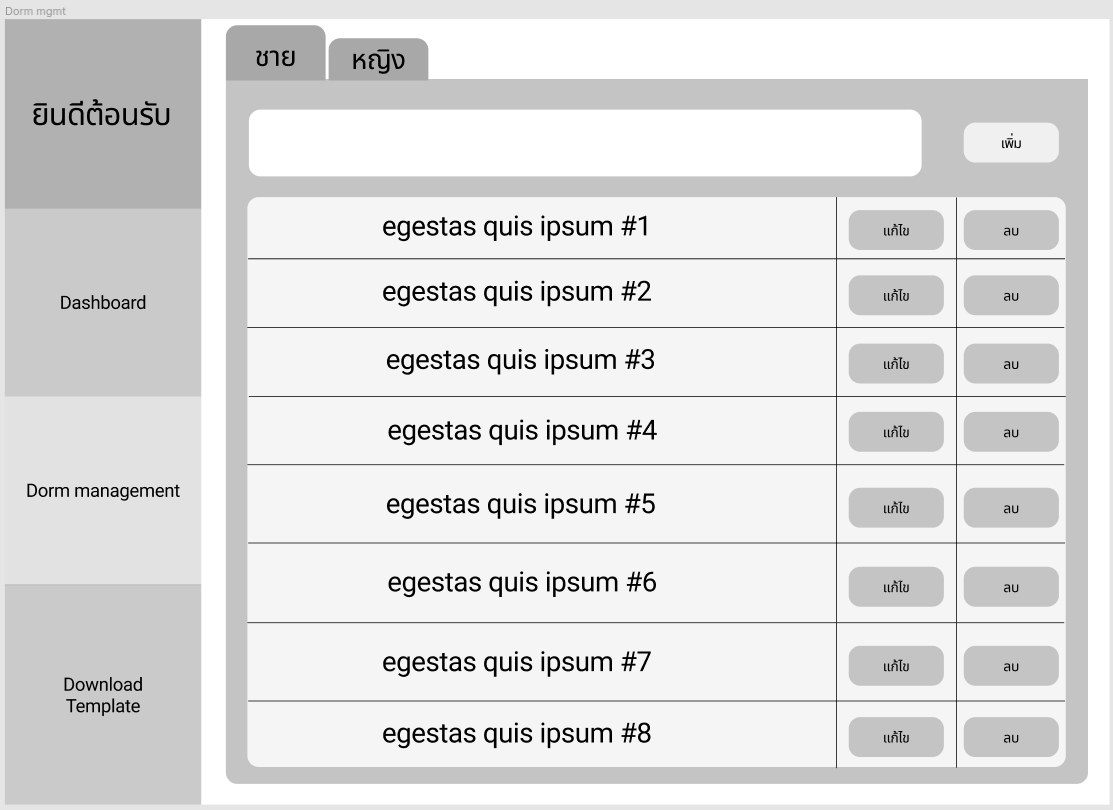
\includegraphics[width=\linewidth]{photo/dormmgmt.png}
  \end{center}
  \caption{หน้าการจัดการหอพักของระบบจอง}
  \label{fig:mgmt}
  \end{figure}
  \begin{figure}[h]
  \begin{center}
  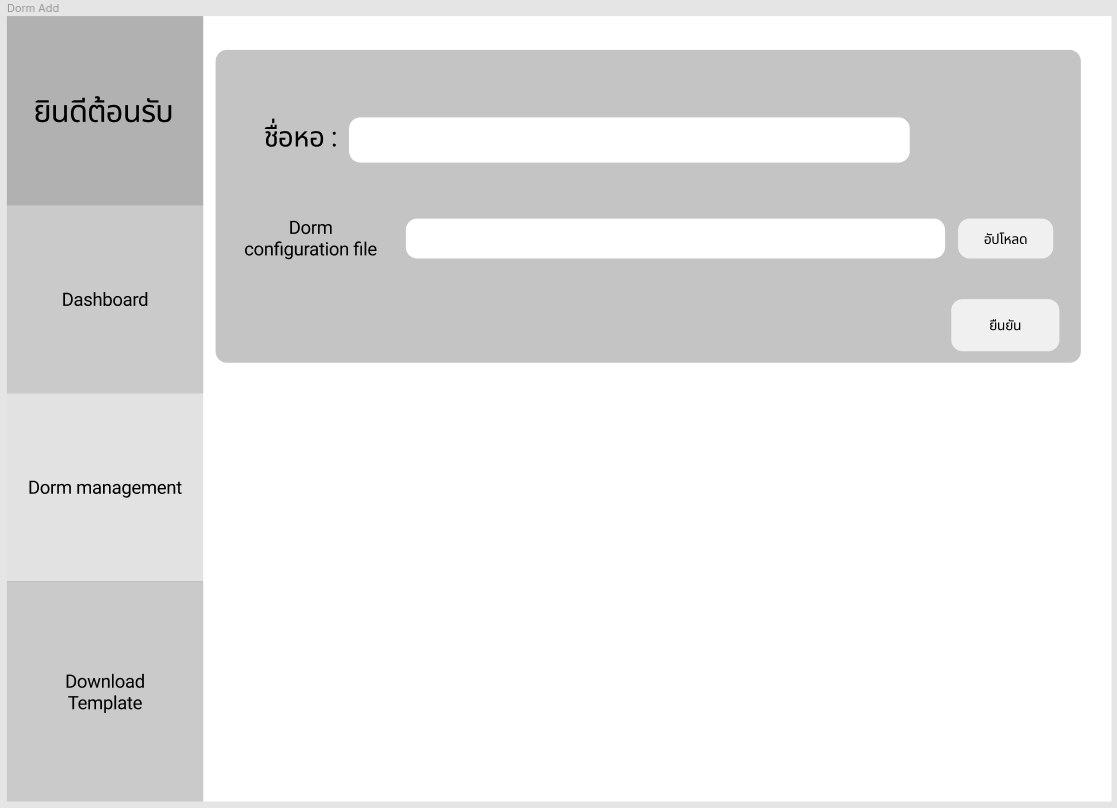
\includegraphics[width=\linewidth]{photo/dormadd.png}
  \end{center}
  \caption{หน้าการเพิ่มหอพักในระบบลงทะเบียน}
  \label{fig:add-dorm}
  \end{figure}
  \begin{figure}[h]
    \begin{center}
    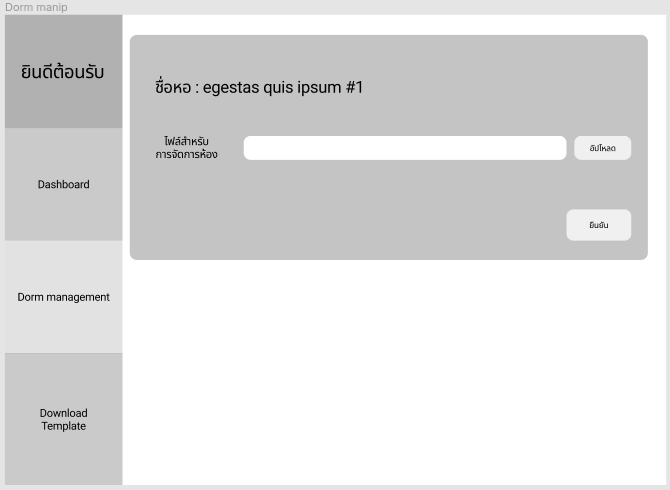
\includegraphics[width=\linewidth]{photo/roommgmt.png}
    \end{center}
    \caption{หน้าการจัดการเพิ่มลดห้องที่เปิดในระบบลงทะเบียน}
    \label{fig:room-mgmt}
    \end{figure}
  
  \clearpage
  \item ระบบศูนย์รวมไฟล์แม่แบบของระบบลงทะเบียน: ให้ผู้ดูแลระบบสามารถเข้ามาดาวน์โหลดไฟล์แม่แบบที่ต้องใช้ในการจัดการระบบฐานข้อมูล\CIreply{mention template}
        ยกตัวอย่างเช่น ไฟล์แม่แบบการตั้งค่าห้องพักที่จะเปิดให้ลงทะเบียน ภายในไฟล์จะมีฟอร์มที่มีหัวข้อที่ต้องกรอกจัดเตรียมไว้ให้แล้ว ซึ่งไฟล์ทั้งหมดจะเป็นไฟล์สกุล .csv
  % \CIreply{ดาวน์โหลดไฟล์พวกนี้ไปเพื่ออะไร?}
  \begin{figure}[h]
  \begin{center}
  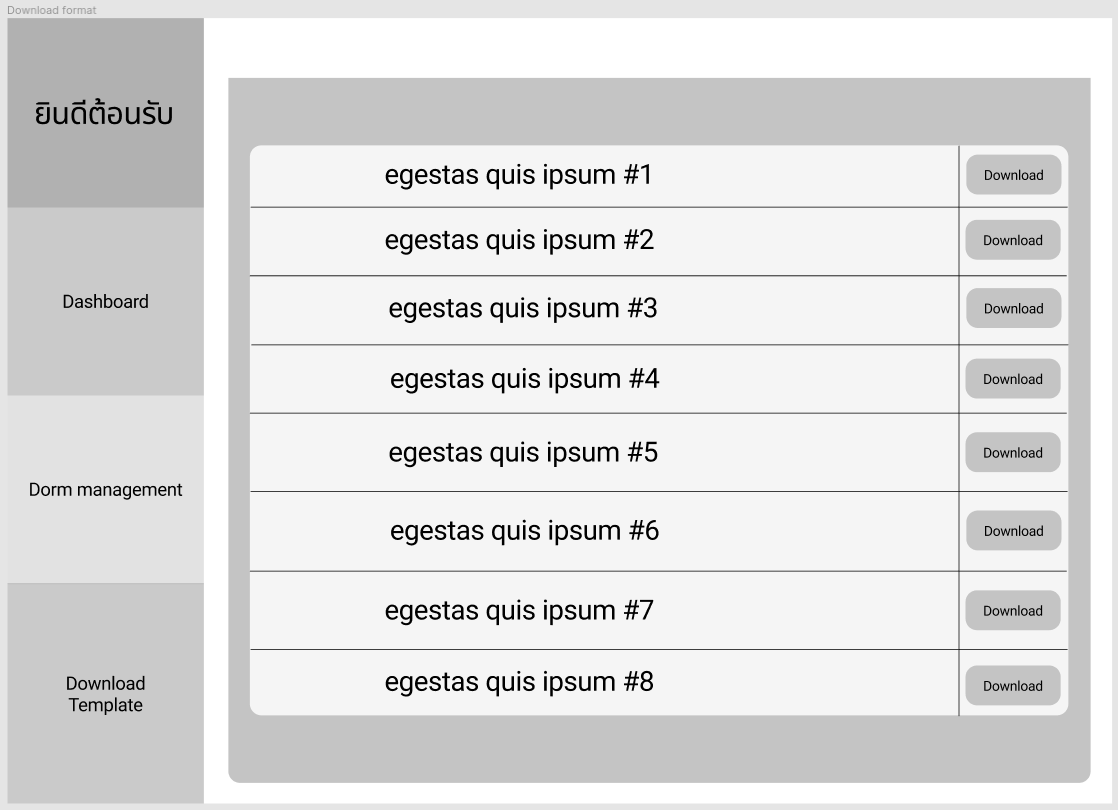
\includegraphics[width=\linewidth]{photo/format.png}
  \end{center}
  \caption{หน้าดาวน์โหลดไฟล์}
  \label{fig:format-db}
  \end{figure}
\end{enumerate}
